\chapter*{What Are Mad Maps?}

\begin{figure}[h]
\centering
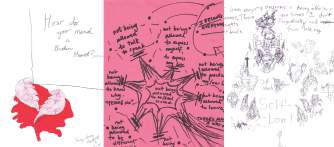
\includegraphics[height=6cm]{TeX_files/0-0.png}
\caption{IMad Maps In Process image courtesy of Sacramento Icarus Project}
\label{2-0}
\end{figure}


In  a  world  that  seals  up  the  side  trails,  hidden  doors  and  underground  caves, forcing  us  all  to  walk  the  arbitrary  straight  path  of  so-called  normalcy,  The Icarus Project is a respite for those who wish to explore the art of getting lost. Fueled  by  hope  and  creativity,  our  members  have  been  artfully  forging  roads and making maps that define our journeys with mental health struggles in the context of a crookedly beautiful world. We have called these cartographic musings Mad Maps.

Mad  Maps  are  documents  that  we  create  for  ourselves  as  reminders  of  our goals, what is important to us, our personal signs of struggle, and our strategies for self-determined well-being. Along  the  way  we’ve  learned  that  our  communities  are  impacted  by  societal systems in different ways, and that these differences affect our mental health. Our  guides  approach  important  issues  such  as  oppression  and  intergenerational trauma and invite you to join others in crafting solutions that help transform the health of our communities.

This  guide  will  help  you  make  your  own  Mad  Map.  Drawing  from  the  input  of hundreds  of  members  of  the  Icarus  Project  community,  it  will  take  you  step by  step  through  the  process  of  creating  your  own  wellness  documents.  The guides help you identify and share what you need for support in times of crisis, with the safety of knowing that you are drawing inspiration from tried and true resources shared by people with lived experiences. We hope you will recognize your own experiences in what others have written--and thus discover language to  describe  your  experiences  and  new  tools  to  maintain  your  well-being  and transform your community.

When  you’re  finished  we’d  love  to  share  your  map  with  the  Icarus  community. By sharing our maps, we can identify our common struggles, inspire each other, teach each other how we can best be supported, and come together to transform the world around us. We envision a world where people create effective  communities  of  support  and  for  individual  and  collective  liberation.  Learn more  about  our  network  of  local  chapters,  upcoming  workshops  and  events, and  how  you  can  join  the  radical  mental  health  movement  at  www.theicarusproject.net.


\noindent\textcolor{ProcessBlue}{\textbf{\LARGE{How To Use This Guide}}}\\

It’s best to work through this guide from front to  back. At each step we’ll provide answers Icarus members gave to a set of questions you can use as inspiration for your own. Check all that apply. In the back you’ll also find the same 15 questions and space to write your own.

Some  people  find  reading  about  the  experiences  of  others  helps  them  better document  their  own,  while  others  know  what  they  want  to  say  without  any prompting.  Either  way,  or  somewhere  in  between,  is  OK.  There  is  no  right  or wrong. In fact, you can even use this guide more than once as your life changes and you have new experiences. Similarly, writing our answers is just one way of mapping. Some people only use words in their maps, while others use art or diagrams.  You  might  use  the  questions  to  start  exploring  and  then  find  you’d like to map in a different way. We just want you to find whatever works best for you to tell your own story.

There are four sections in this guide. In Section I and II  you’ll find an introduction to oppression--what it is and how we experience it. Section III explores how we  cope  with  it.  Section  IV  asks  how  we  can  address  oppression  in  our  communities and achieve collective liberation. The Epilogue is where you’ll find the questions and room to answer them to make your own map.

By the time you’re finished you’ll have a greater awareness of how oppression affects  you and those around you. You’ll also create your own Mad Map, which serves as a reminder document for yourself and the people around you about your wellness goals, warning signs, strategies for health, and who you trust to look out for your best interests when you’re struggling.

Each  section  is  designed  for  people  at  any  stage  of  life--whether  you’re  just starting to examine “madness” and oppression or you’re looking for additional tools  to  identify  needs  and  achieve  your  goals.  We  hope  everybody  will  find inspiration and strategies that best suit their needs and those of their communities  in  this  guide.  Most  importantly,  we  hope  that  we  can  all  feel  less  alone and find hope in a harsh world through making our own maps.

Please  note  that  reading  about  oppression  and  harm  can  sometimes  be  triggering in and of itself. Take care of yourself as you work your way through this text by making sure you’re in a safe place where you can make adjustments for your safety and comfort as needed. Take breaks, breathe, sing, exercise, call a friend, take a nap, or engage in other kinds of care that nourishes you. Remember, you are worthy of love and you are part of a whole international community of people who are on this healing journey together.

\begin{figure}[h]
	\centering
	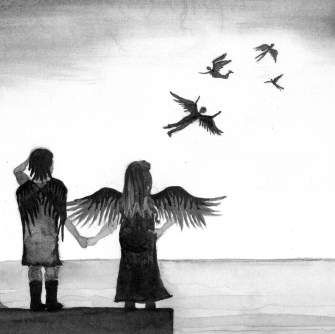
\includegraphics[height=12cm]{TeX_files/0-1.png}
	\caption{Artist: Jacks McNamara}
	\label{2-0}
\end{figure}
